\documentclass[11pt,a4paper,titlepage, ngerman]{article}

\usepackage[utf8]{inputenc}	% Diese Pakete sind
\usepackage[T1]{fontenc}		% für die Verwendung 
\usepackage{ngerman}			% von Umlauten im tex-file
\usepackage{lmodern}			% Schriftart, die am Bildschirm besser lesbar ist
\usepackage{graphicx}			% Zum Einbinden von Formeln
\usepackage{url}					% Zur Darstellung von Webadressen
\usepackage{siunitx}
\usepackage{amsmath}			% für equation*
\usepackage{subcaption}
\usepackage{wrapfig}

\begin{document}
%	\setlength{\parindent}{0em} 
	
	\begin{titlepage}
		\centering
		{\scshape\LARGE Versuchsbericht zu \par}
		\vspace{1cm}
		{\scshape\huge E4 -- Kennlinien\par}
		\vspace{2.5cm}
		{\LARGE Gruppe 10 Mi\par}
		\vspace{0.5cm}
		{\large Alex Oster (E-Mail: a\_oste16@uni--muenster.de) \par}
		{\large Jonathan Sigrist (E-Mail: j\_sigr01@uni--muenster.de ) \par}
		\vfill
		durchgeführt am 8.11.2017\par
		betreut von\par
		{\large David \textsc{Pahl}}
		
		\vfill
		
		{\large \today\par}
	\end{titlepage}
		
	\tableofcontents
	
	\newpage
	
	\section{Kurzfassung}
		
		In diesem Bericht befassen wir uns mit Kennlinien. Eine Kennlinie ist die Kurve, die entsteht, wenn man die Spannung gegen den Strom aufträgt. Aus dem Ohm'schen Gesetz $U=RI$ bzw. $I = \frac{1}{R}U $ ergibt sich, dass diese durch den Widerstand dargestellt wird. 
		
		Wir betrachten im Folgenden zwei Versuchen, die uns verschiedenen Arten von Widerständen näher bringen sollen. 
		
		In dem ersten Versuch betrachten wir fünf verschiedene Arten von Widerständen. Eine einfache Diode, eine Zenerdiode, einen NTC-Widerstand, eine Glüh- und eine Glimmlampe. Wir messen hierbei den Strom in Abhängigkeit von der Spannung und werten die Ergebnisse aus. Dazu gehen wir auf die Funktionsweise von (dotierten) Halbleitern und Gasentladungen ein. 
		
		Die Abhängigkeit des Widerstands von der Temperatur wird dann in dem zweiten Versuch betrachtet.
		Hierzu erhitzen wir einen Kupferdraht in Öl, lassen ihn danach abkühlen und messen durchgehend seinen Widerstand mit Hilfe einer Wheatstone'schen Brücke. Unsere Ergebnisse für den Kupferdraht verknüpfen wir dann mit der elektrischen Leitfähigkeit von Metallen.

	\section{Versuch 1: Strom-Spannungs-Charakteristik}
		
		In diesem Versuch betrachten wir die Kennlinien von verschiedenen Bauteilen. Dafür messen wir den Strom und tragen diesen gegen unsere Eingangsspannung auf. Den sich daraus ergebenen Verlauf, die Kennlinie, erklären wir dann im Sachverhalt. 
		
		\subsection{Methoden} 
		
		Der Versuchsaufbau ist In Abb. \ref{Schaltskizze1} skizziert. Dabei fließt der Strom nur über jeweils einen Aufbau. 
		
		Da die Spannungsquelle keine genaue Angabe der Eingangsspannung liefert, messen wir diese mit einem Multimeter, welches parallel zu dem Aufbau geschaltet ist. Den Strom hingegen messen wir mit einem zweiten Multimeter, welches in Reihe zu dem Aufbau geschaltet ist.
		
		Für die Teilversuche a) bis d) verwenden wir Eingangsspannungen im Bereich von \SIrange{0}{20}{\V} und für die Glimmlampe in e) Eingangsspannungen von \SIrange{0}{150}{\V}.
		
		\begin{figure}
			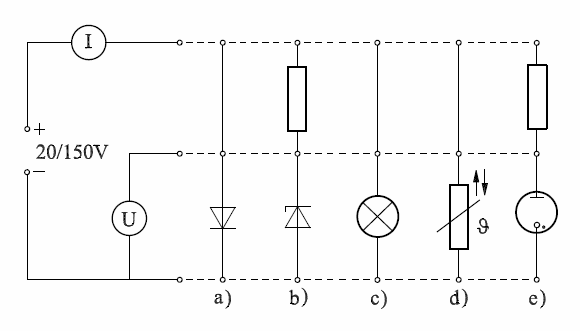
\includegraphics[width=\textwidth]{Versuch1.png}
			\caption{Schaltskizze zu Versuch 1}
			\label{Schaltskizze1}
		\end{figure}

		\subsection{a) Diode in Durchlassrichtung} 
			\label{a)}
			
			\subsubsection{Diode}
				\label{Diode}
				
				Eine Diode ist ein Bauteil, mit dem Spannungen nur von einer Richtung durchgelassen werden. Diesen Effekt erhält man, wenn man einen Halbleiter mit einem Element aus der dritten Hauptgruppe dotiert (p-Leiter) und einen anderen mit einem Element aus der fünften Hauptgruppe (n-Leiter) und diese aneinander grenzen lässt. Hierbei entsteht eine Raumladungszone im Übergangsbereich, da die Elektronen des n-Leiters zu dem p-Leiter wandern. Da in dem Übergangsbereich weniger freie Ladungsträger sind, als im restlichen Leiter, nimmt die Leitfähigkeit an dieser Stelle stark ab.
				
				Legt man den positiven Pol einer aüßeren Spannung an den n-Leiter an, so vergrößert sich der Übergangsbereich. Bei einem negativen Pol hingegen, verkleinert sich dieser, sodass der Strom durch den Leiter fließen kann. 
			
			\subsubsection{Messung}
				
				Unsere Messwerte ergaben, wie in Abb. \ref{KL a} zu sehen ist, dass die Kennlinie bei einer Diode in Durchflussrichtung exponentiell verläuft. Einen messbaren Strom erhielten wir erst ab ca. \SI{0.5}{\V} und es ließen sich ab ungefähr \SI{0.72}{\V} keine weiteren Werte messen. 
				
				\begin{figure}
					\centering
					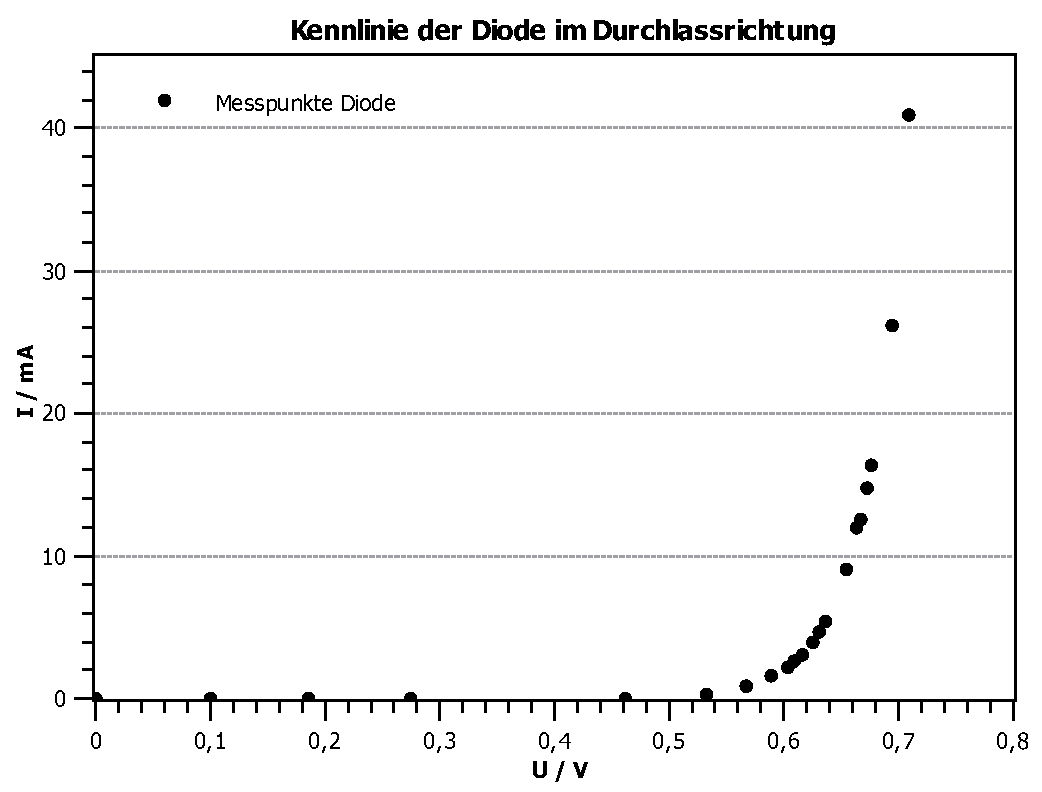
\includegraphics[width=\textwidth]{KennlinieDiode.pdf}
					\caption{Messung zu Versuch 1a)}
					\label{KL a}
				\end{figure}
			
			\subsubsection{Schlussfolgerung}
			
				Unsere Ergebnisse deuten darauf hin, dass mindestens \SI{0.5}{\V} nötig sind, um den Übergangsbereich, der Diode, so zu verkleinern, dass ein Strom fließen kann. 
				
				Dass sich ab ca. \SI{0.72}{\V} keine weiteren Werte messen ließen, könnte daran liegen, dass die Diode, so modifiziert ist, dass nicht mehr Spannung als diese \SI{0.72}{\V} durchgelassen werden können. Somit geht der Widerstand nicht gegen null und wir vermeiden einen Kurzschluss.
				
				Die Größe des Übergangsbereichs steht in direktem Zusammenhang mit dem Widerstand.  Denn je mehr Spannung anliegt, desto kleiner wird der Übergangsbereich und umso leichter können freie Ladungsträger diesen Bereich passieren. Der Widerstand wird also geringer.
				
				Diesen Sachverhalt stützt der exponentielle Verlauf, der von uns gemessenen, Kennlinie. Demnach entspricht unser Ergebnis den Erwartungen.
				
		\subsection{b) Zenerdiode} 
			
			Die Zenerdiode funktioniert wie die in \ref{Diode} beschriebene Diode, nur dass bei der Zenerdiode auch in Sperrrichtung Strom fließen kann, insofern die angelegte Spannung groß genug ist. Dies geschieht durch das Kleiner-werden der Potentialbarrieren bei hochdotierten p-n-Übergängen, wenn starke Ströme fließen. Hierbei kommt es zu dem quantenmechanischen Tunneleffekt, der dazu führt, dass Valenzelektronen in das Leitungsband gelangen. Es bildet sich ein Durchbruchstrom.
			
			\subsubsection{Messung}
			
				 \begin{itemize}
				 	
				 	\item Sperrrichtung: 
				 	
				 	In Abb. \ref{KL b1} erkennt man, dass wir auch hier einen exponentiellen Verlauf der Kennlinie gemessen haben. 				 	
				 	Anders als in der vorausgehenden Messung, fließt hier jedoch erst ab ca. \SI{2.6}{\V} ein Strom und wir konnten dieses mal bis ungefähr \SI{5}{\V} einen Strom messen.
				 	
				 	\begin{figure}
				 		\centering
				 		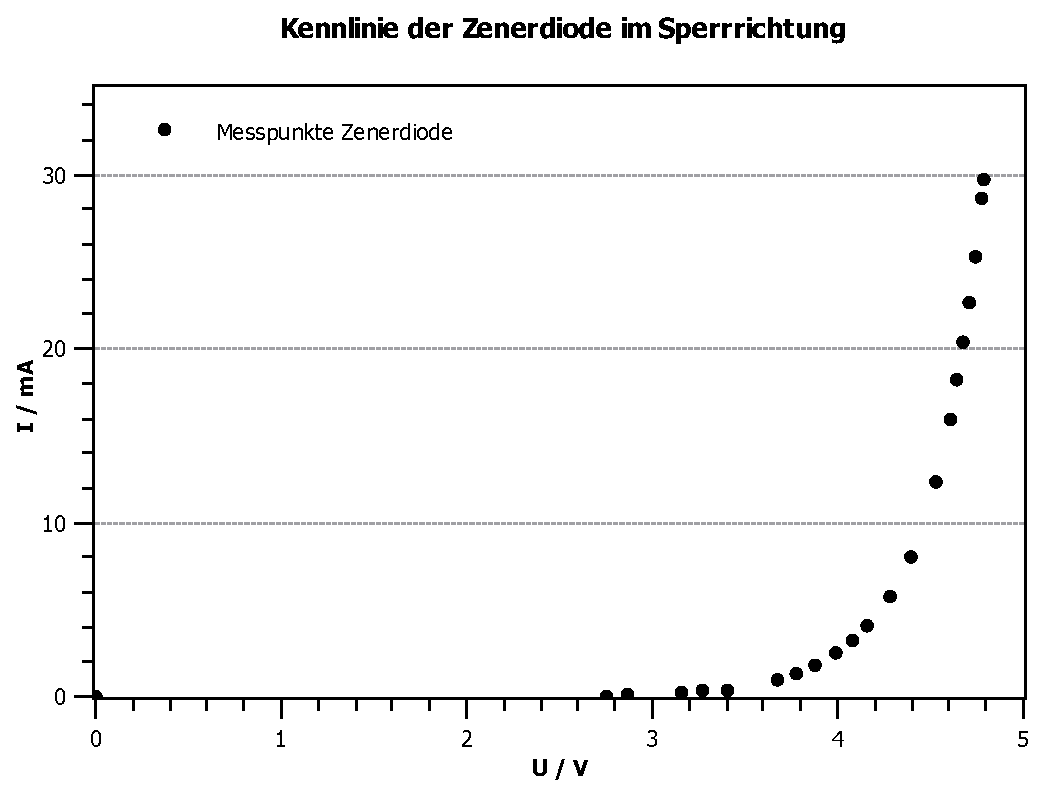
\includegraphics[width=\textwidth]{KennlinieZenerdiodeSperrrichtung.pdf}
				 		\caption{Erste Messung zu Versuch 1b)}
				 		\label{KL b1}
				 	\end{figure}
				 	
				 	\item Durchlassrichtung:  
				 	
				 	Diese Messung verlief analog zu der in \ref{a)} durchgeführten Messung, wie in Abb. \ref{KL b2} zu sehen. Verglichen mit der ersten Messung, ist diese genauer und der zu erkennende exponentielle Anstieg wirkt ein wenig stärker.
				 	
				 	\begin{figure}
				 		\centering
				 		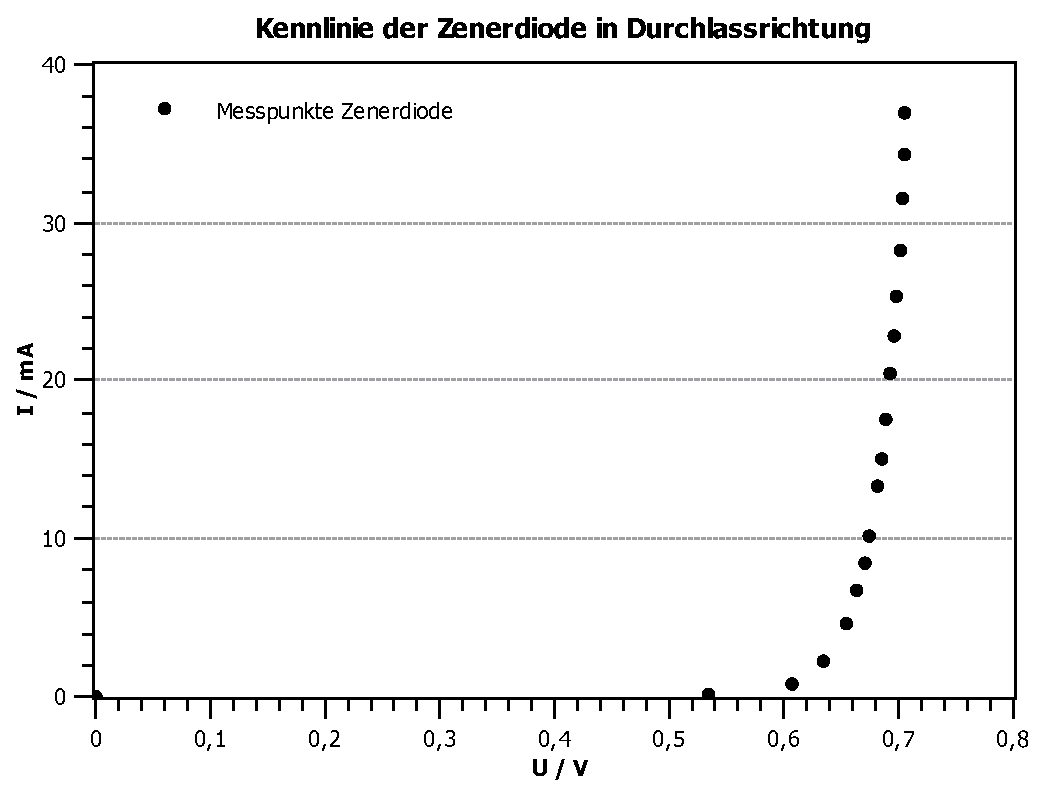
\includegraphics[width=\textwidth]{KennlinieZenerdiodeDurchlassrichtung.pdf}
				 		\caption{Zweite Messung zu Versuch 1b}
				 		\label{KL b2}
				 	\end{figure}
				 					 	
				\end{itemize}
											
			\subsubsection{Schlussfolgerung}
				
				Die Ergebnisse dieser Messung bezüglich der Durchlassrichtung stehen in direktem Zusammenhang zu dem Ergebnis aus \ref{a)}. 
				Für die Sperrrichtung hingegen ermitteln wir, dass die Benötigte Spannung für einen Stromfluss bei ca. \SI{2.6}{\V} liegt. 
				
				Verglichen mit den \SI{0.5}{\V} in Durchflussrichtung ist dies ein beachtlicher und zu erwartender Unterschied. Im Gegenzug zu der Verkleinerung des Übergangsbereichs der Diode fließt in Sperrrichtung, wenn überhaupt, nur der Durchbruchstrom und für diesen benötigt man hohe Spannungen. 
				
				Dass auch in Sperrrichtung die Kennlinie exponentiell verläuft, hat einen ähnlichen Grund, wie in Durchflussrichtung. Denn je höher die Spannung, desto mehr Elektronen lösen sich aus dem Valenzband des p-Leiters und umso stärker ist folglich der Durchbruchstrom. Der Widerstand wird also auch hier mit höherer Spannung kleiner. 
				
		\subsection{c) Glühlampe} 
			
			Bei der Glühlampe fließt der Strom durch einen Glühdraht, dieser erwärmt sich dabei und beginnt zu glühen. Wir betrachten also nun, wie sich der Widerstand nach Inbetriebnahme der Glühlampe ändert. Dazu messen wir, wie bisher, den Strom und tragen ihn gegen die Spannung auf. Um die Änderung des Widerstandes besser zu betrachten tragen wir zudem noch den Widerstand gegen die Spannung aus, wobei sich dieser aus dem Ohm'schen Gesetz und der vorausgegangen Strommessung ergibt.  
			
			\subsubsection{Messung}
				
				Die Kennlinie der Glühlampe verläuft zunächst krumm, richtet sich im späteren Verlauf jedoch annähernd linear aus. Wir beobachten, dass die Glühlampe ab ca. \SI{2.6}{\V} anfängt schwach zu glühen. In Abb. \ref{KL c} ist zu sehen, dass die Kennlinie sich in diesem Bereich beginnt sich linear auszurichten.
				
				Der letzte messbare Wert war hier bei ca. \SI{7.2}{\V}
				
				\begin{figure}
					\centering
					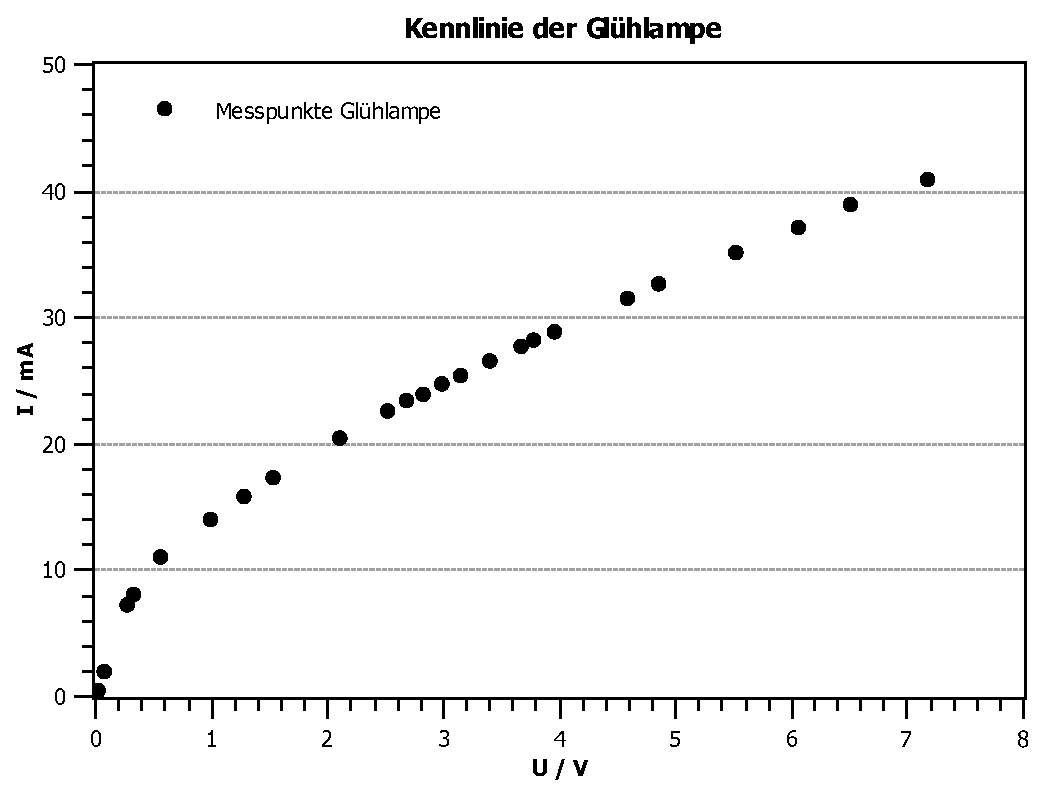
\includegraphics[width=\textwidth]{KennlinieGluehlampe.pdf}
					\caption{Messung zu Versuch 1c)}
					\label{KL c}
				\end{figure}
				\begin{figure}
					\centering
					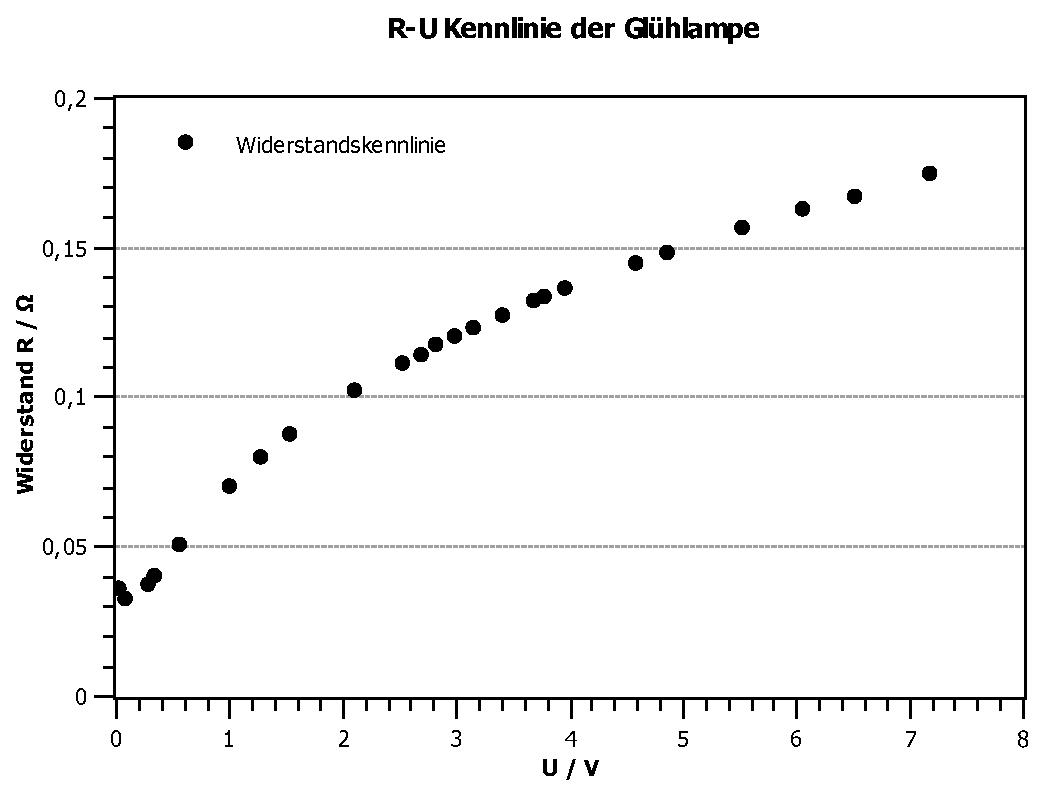
\includegraphics[width=\textwidth]{KennlinieGluehlampeWiderstand.pdf}
					\caption{Widerstand in Abhängigkeit der Spannung}
					\label{R c}
				\end{figure}
			
			\subsubsection{Schlussfolgerung}
			
				Der annähernd lineare Verlauf der Kennlinie deutet darauf hin, dass der Widerstand sich, bei höheren Spannungen, kaum ändert. In Abb. \ref{R c} erkennen wir auch, dass dies der Fall ist, wobei der Widerstand weiterhin langsam steigt.
				
				Das Steigen des Widerstands lässt sich auf die steigende Temperatur zurückführen. Bei dem Glühdraht handelt es sich um ein Metall, vermutlich Wolfram. Metalle haben die Eigenschaft, dass ihre elektrische Leitfähigkeit mit steigender Temperatur abnimmt.
				
				Zu Beginn ist der Glühdraht bei Zimmertemperatur und wie in den beiden Abbildungen zu erkennen ist, steigt der Widerstand zunächst stark, weswegen die Kennlinie erst krumm verläuft. Ab dem Punkt, an dem der Draht glüht, steigt der Widerstand langsamer, da die Temperaturunterschiede schwächer werden.
				
				Dieses Verhalten stimmt mit der Änderung der elektrischen Leitfähigkeit von Metallen bei erhöhten Temperaturen überein.
				
		\subsection{d) NTC-Widerstand} 
			
			NTC-Widerstände bestehen aus Halbleitern und verhalten sich, was den Innenwiderstand betrifft, anders als Metalle. Das \glqq NTC\grqq  steht für \glqq Negative Temperature Coefficient\grqq , soll also heißen, dass sie bei erhöhten Temperaturen, im Gegensatz zu Metallen, besser den elektrischen Strom leiten als bei geringeren Temperaturen.
			
			Bei dieser Messung betrachten wir einen solchen NTC-Widerstand. Bevor wir einen Messwert aufnehmen, lassen wir den Widerstand kurz in Ruhe, so dass er sich auf die Temperatur einstellt, die er bei gegebener Spannung annehmen sollte. 
			
			\subsubsection{Messung}
			
				In Abb. \ref{KL d} sehen wir ähnlich zu den Dioden einen exponentiellen Verlauf der Kennlinie, wobei dieser Widerstand von Anfang an den Strom durchlässt und nicht erst ab einer gewissen Spannung.
				Hier konnten wir nur Werte bis \SI{8}{\V} Eingangsspannung aufnehmen.
				
				\begin{figure}
					\centering
					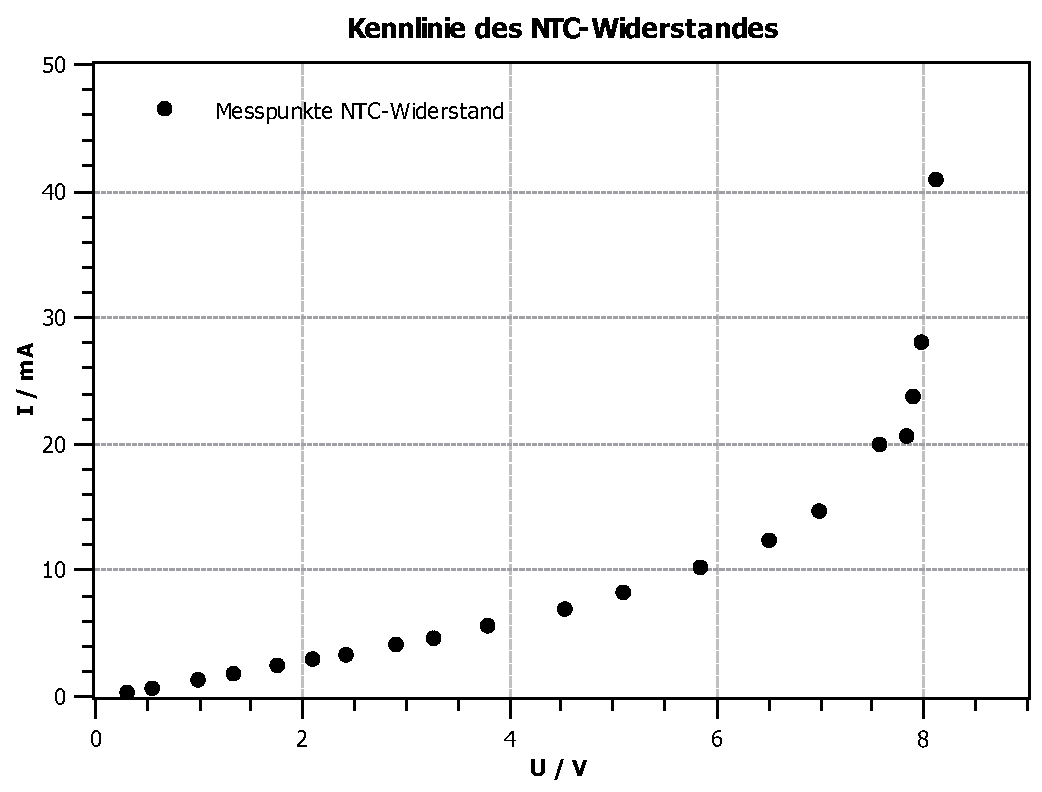
\includegraphics[width=\textwidth]{KennlinieNTCsubgitter.pdf}
					\caption{Messung zu Versuch 1d)}
					\label{KL d}
				\end{figure}
			
			\subsubsection{Schlussfolgerung}
			
				Hier ist klar zu erkennen, dass der Widerstand mit steigender Temperatur (durch steigende Spannung) sinkt, was für NTC-Widerstände charakteristisch ist. 
				
				Dass wir auch hier nicht mehr als bis zu \SI{8}{\V} Eingangsspannung messen konnten, wird ebenfalls aufgrund von Kurzschlussvermeidung gewesen sein.
			
		\subsection{e) Glimmlampe} %Erklärung Glimmlampe, Messung und Schlussfolgerung
			
			\subsubsection{Gasentladungen}
			
				%TODO Glimmlampenfunktionsweise
					
			\subsubsection{Messung}
			
				%TODO Kurve beschreiben
			
				\begin{figure}
					\centering
					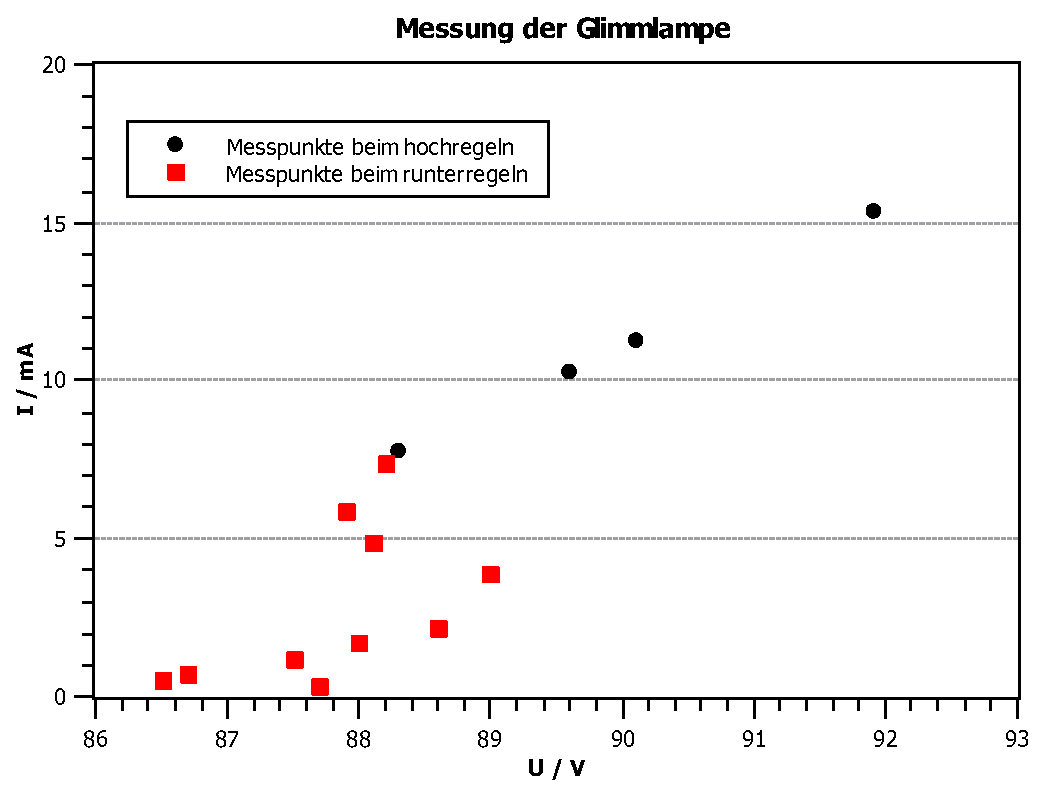
\includegraphics[width=\textwidth]{KennlinieGlimmlampe.pdf}
					\caption{}
					\label{}
				\end{figure}
			
			\subsubsection{Schlussfolgerung}
			
				%TODO Schlussfolgerung
			
	\section{Versuch 2: Widerstand in Abhängigkeit der Temperatur}		

		\subsection{Methoden} %Aufbau und wie/was gemessen wird
		
			%TODO Wheatstone'sche Brücke erklären
			
			\begin{figure}
				\centering
				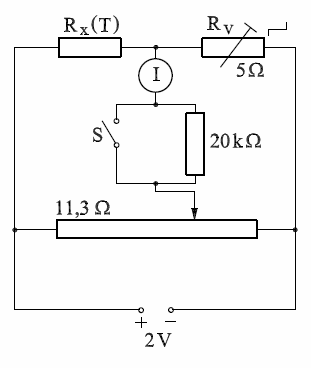
\includegraphics[width=0.6\textwidth]{Versuch2.png}
				\caption{Schaltskizze zu Versuch 1}
				\label{Schaltskizze2}
			\end{figure}
		
		\subsection{Messung}
			
			%TODO Kurve beschreiben
			
				\begin{figure}
				\centering
				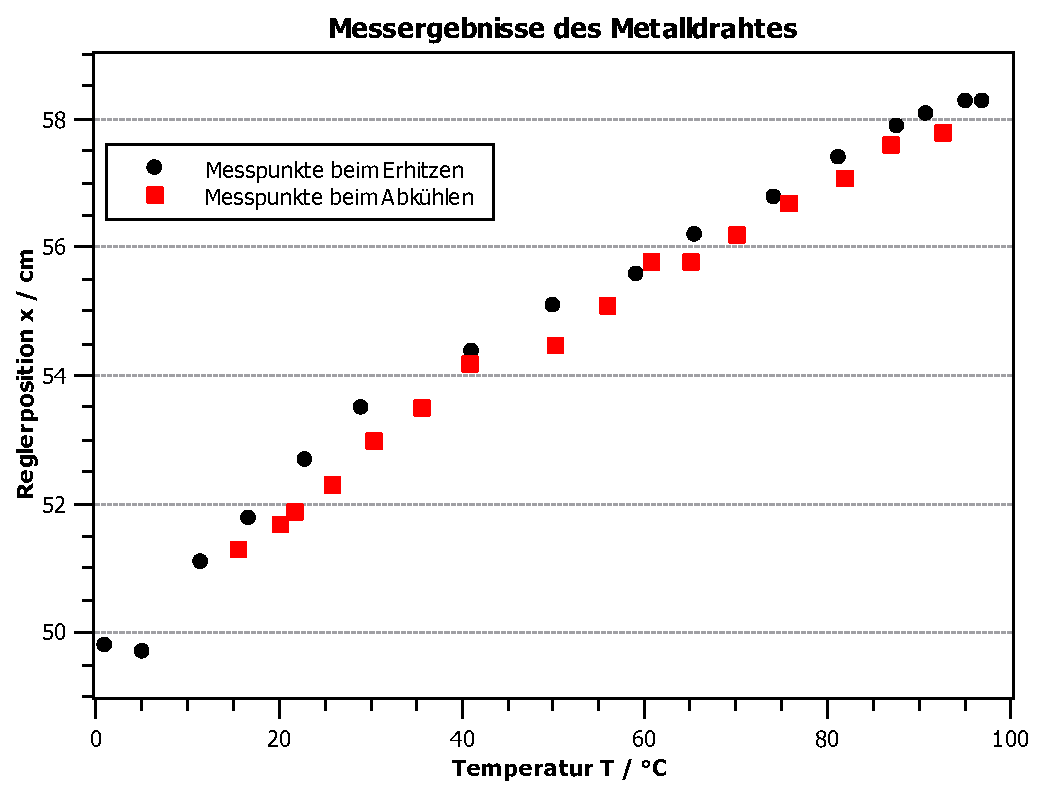
\includegraphics[width=\textwidth]{MessungDraht.pdf}
				\caption{}
				\label{}
			\end{figure}
			
		\subsection{Schlussfolgerung}	
			
			%TODO Schlussfolgerung	
	
	\newpage	
	\begin{thebibliography}	
		e empty
	\end{thebibliography}	
			
\end{document} 